\normalsize
\subsection{Colocated Spatial Discretization}
The model with colcated spatial discretization defines all the scalar variables and velocities in the cell center of a Cartesian grid system. To simplify the notation, the subscript ($i, \ j, \ k$) means that the value is located at $(x,y,z)=[  (i-\f{1}{2}) \Delta x, (j-\f{1}{2}) \Delta y, (k-\f{1}{2})\Delta z ]$.
\begin{figure}[h]
\hspace{0.4in}
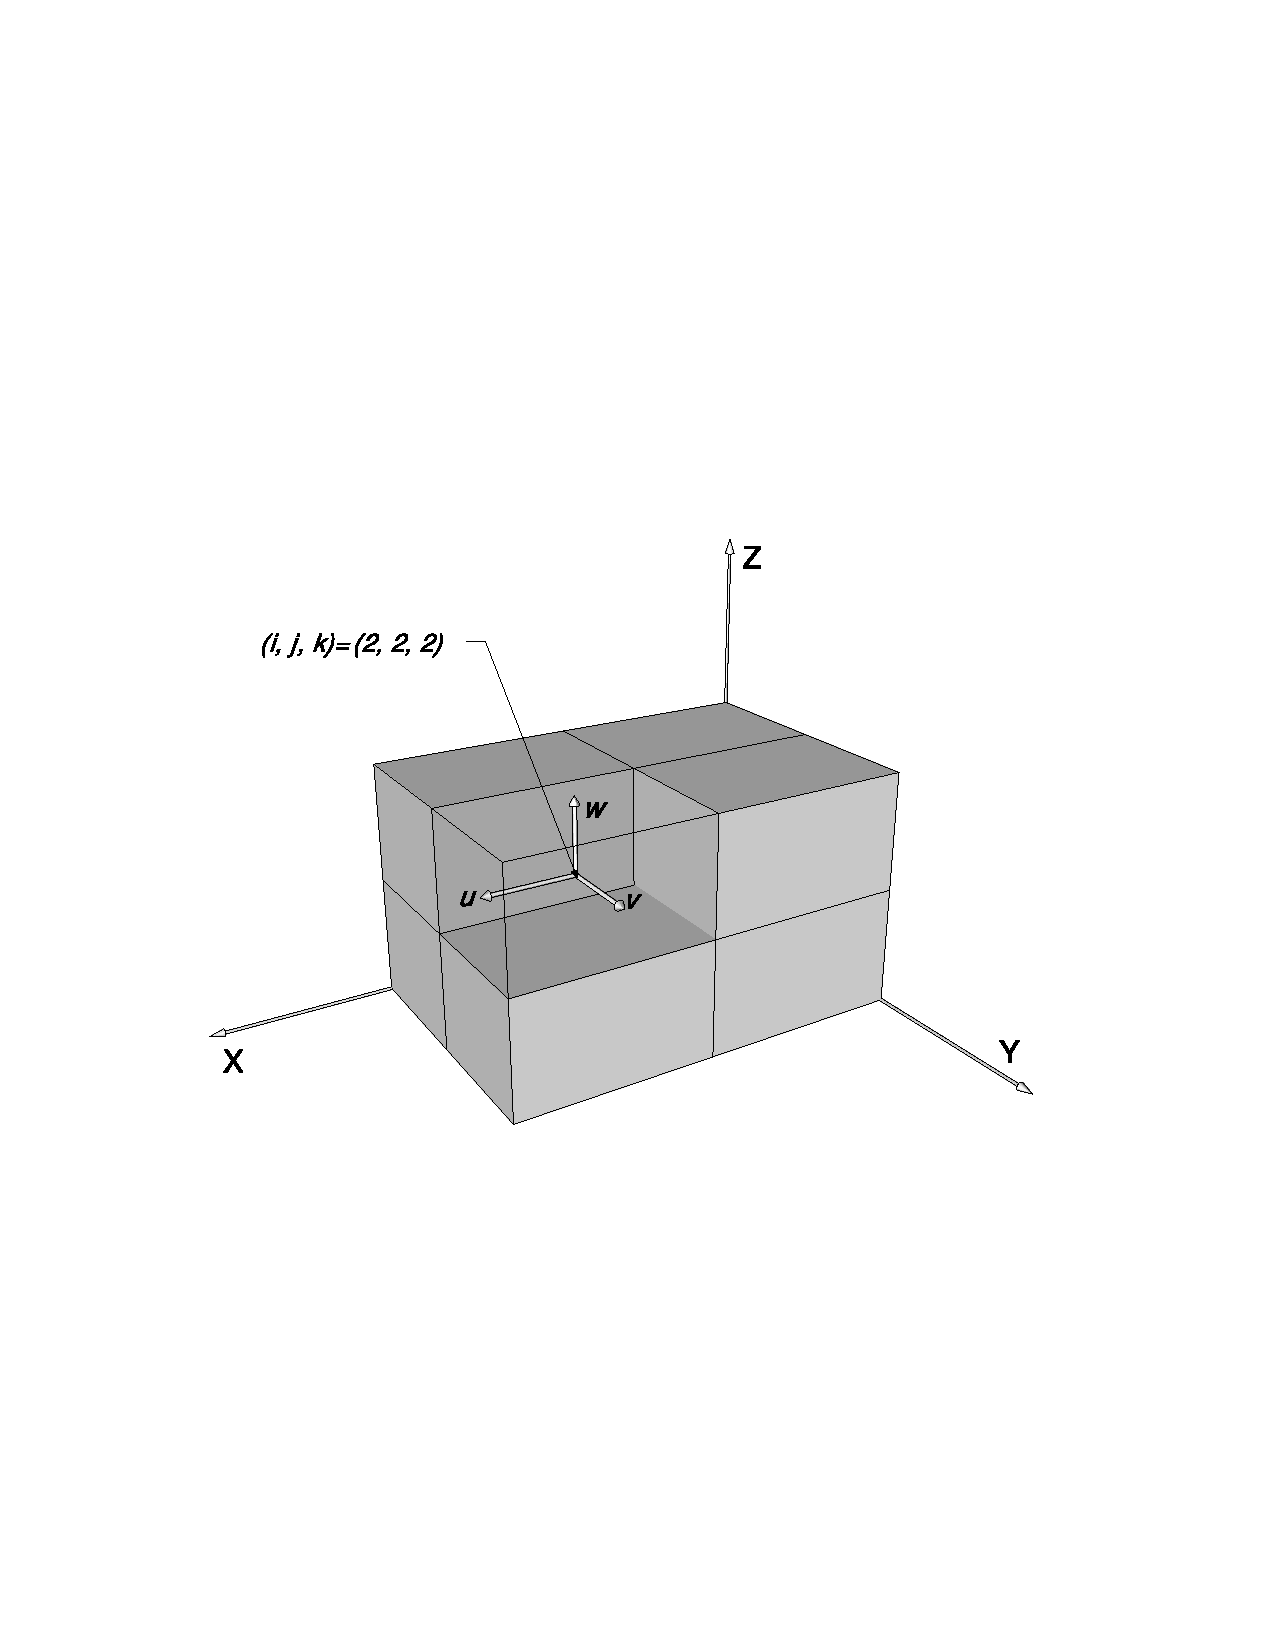
\includegraphics[width=4.7in]{../figures/Colocated/Colocated3D.pdf}
\label{fig:Colocated3D}
\caption{Colocated grid.}
\end{figure}
\begin{figure}[htbp]
\hspace{1.8in}
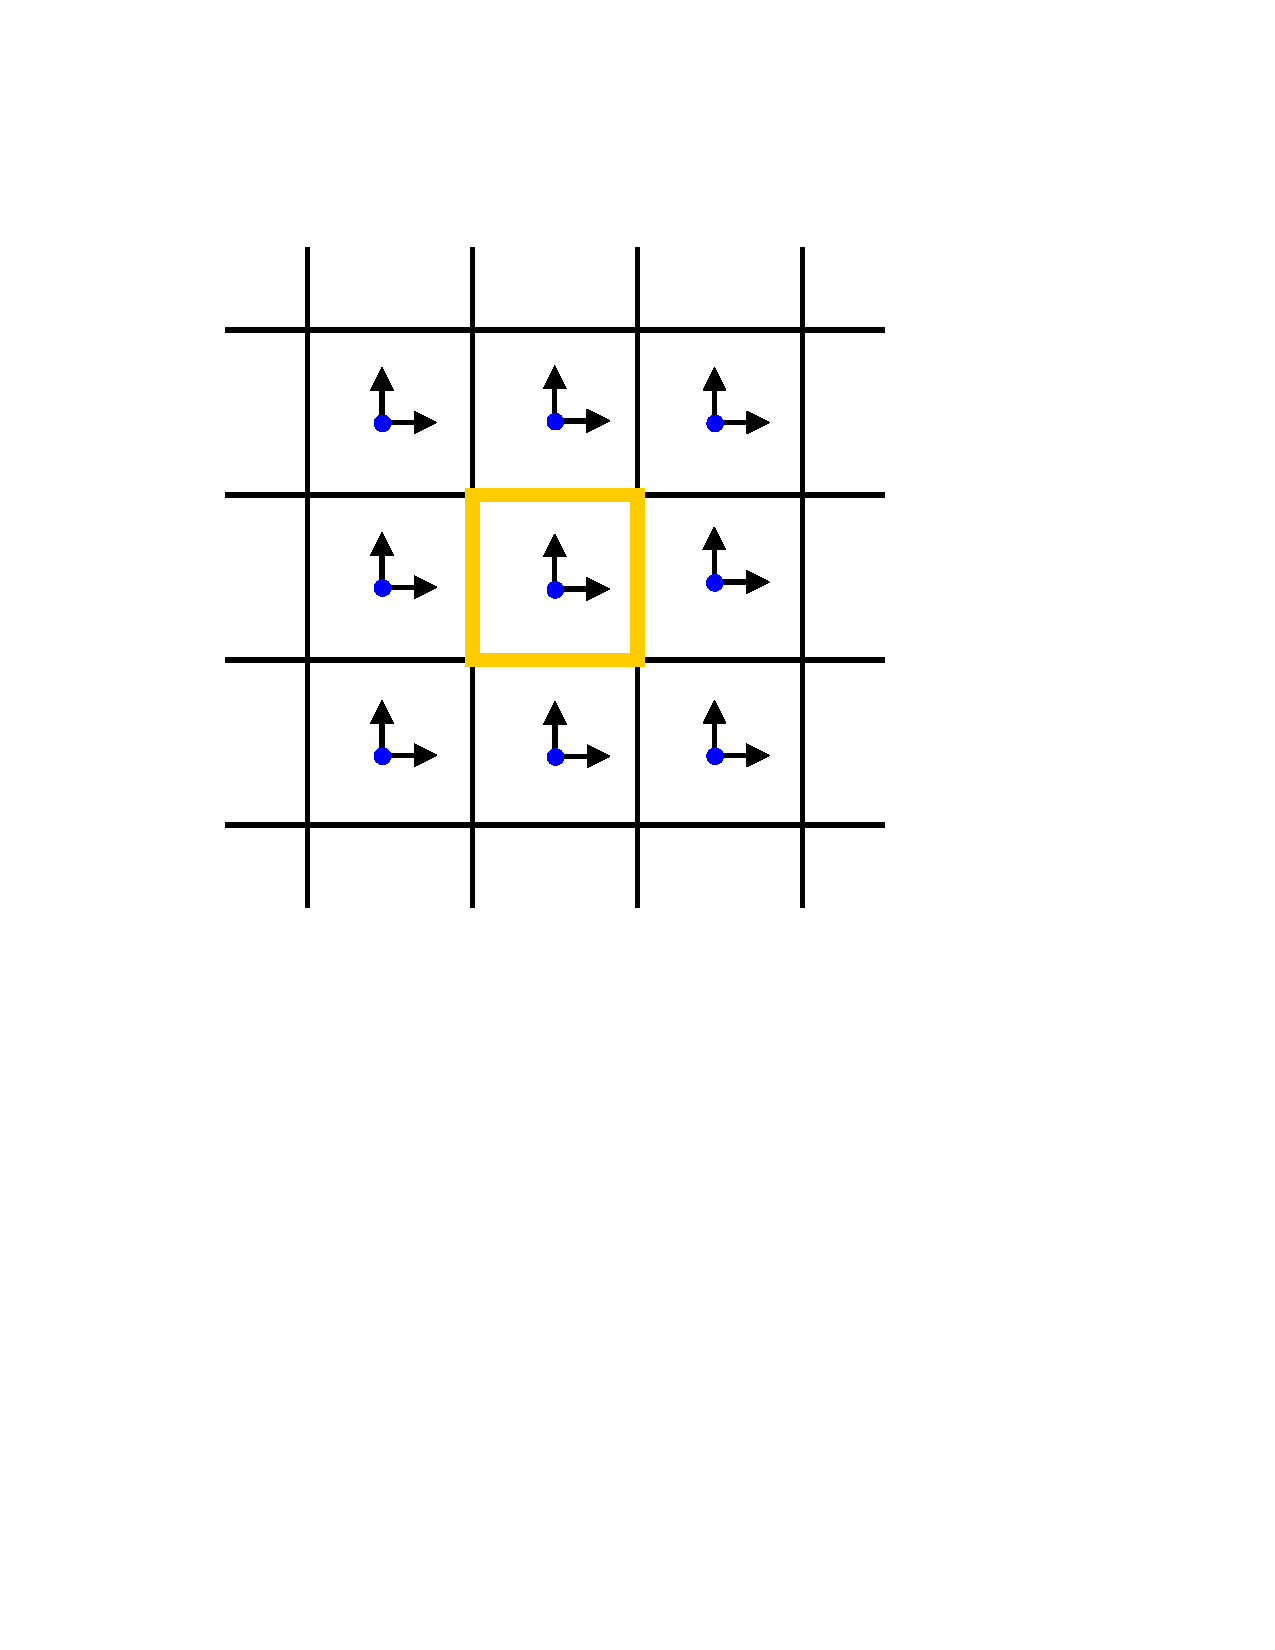
\includegraphics[scale=0.50]{../figures/Grids/Colocated-CV.pdf}
\label{fig:Staggered-CV-w}
\caption{Control volume of the colocated grid.}
\end{figure}
With the location of the value denoted by the subscript, Equation \ref{eqn:chap-FlowModel-momentum-u}, \ref{eqn:chap-FlowModel-momentum-v}, and \ref{eqn:chap-FlowModel-momentum-w} can be discretized as:
\begin {eqnarray}
u_{i,j,k}^{*} &=& u_{i,j,k}^{n}+ \Delta t
\{ -A(u_{i,j,k}^n)+E(u_{i,j,k}^n) \nonumber \\
&-&B(u_{i,j,k}^n)-g\frac{h_{i+1,j,k}^n-h_{i-1,j,k}^n}{2\Delta x}
-\frac{1}{\rho}\frac{p_{d \ i+1,j,k}^n-p_{d \ i-1,j,k}^n}{ 2\Delta x}
\}
\end{eqnarray}
\begin {eqnarray}
v_{i,j,k}^{*} &=& v_{i,j,k}^{n}+ \Delta t
\{ -A(v_{i,j,k}^n)+E(v_{i,j,k}^n) \nonumber \\
&-&B(v_{i,j,k}^n)-g\frac{h_{i,j+1,k}^n-h_{i,j-1,k}^n}{2\Delta y}
-\frac{1}{\rho}\frac{p_{d \ i,j+1,k}^n-p_{d \ i,j-1,k}^n}{ 2\Delta y}
\}
\end{eqnarray}
\begin {eqnarray}
w_{i,j,k}^{*} &=& w_{i,j,k}^{n}+ \Delta t
\{ -A(w_{i,j,k}^n)+E(w_{i,j,k}^n) \nonumber \\
&-&\frac{1}{\rho}\frac{p_{d \ i,j,k+1}^n-p_{d \ i,j,k-1}^n}{ 2\Delta z}
\}
\end{eqnarray}
The advection term is approximated by the central difference,
\begin{eqnarray}
A(u_{i,j,k})&=&( \frac{\partial uu}{\partial x} +  \frac{\partial
uv}{\partial y}+\frac{\partial uw}{\partial z})_{i,j, k}\nonumber\\
&=&\frac{(u^n_{i+\f{1}{2},j,k})^2-(u^n_{i-\f{1}{2},j,k})^2}{\Delta
x}
+\frac{(u^n_{i+\f{1}{2},j,k})(v^n_{i+\f{1}{2},j,k})
-(u^n_{i-\f{1}{2},j,k})(v^n_{i-\f{1}{2},j,k})}{\Delta
y}\nonumber \\
& & +\frac{(u^n_{i+\f{1}{2},j,k})(w^n_{i+\f{1}{2},j,k})
-(u^n_{i-\f{1}{2},j,k})(w^n_{i-\f{1}{2},j,k})}{\Delta z}
\end{eqnarray}
where the velocities on the face of control volumes are:
\begin{eqnarray*}
u_{i+\f{1}{2},j,k}=\f{u_{i,j,k}+u_{i+1,j,k}}{2} &,& \ u_{i-\f{1}{2},j,k}=\f{u_{i,j,k}+u_{i-1,j,k}}{2}\\
v_{i+\f{1}{2},j,k}=\f{v_{i,j,k}+v_{i+1,j,k}}{2} &,& \
v_{i-\f{1}{2},j,k}=\f{v_{i,j,k}+v_{i-1,j,k}}{2}\\
w_{i+\f{1}{2},j,k}=\f{w_{i,j,k}+w_{i+1,j,k}}{2} &,& \
w_{i-\f{1}{2},j,k}=\f{w_{i,j,k}+w_{i-1,j,k}}{2}
\end{eqnarray*}
 The diffusion, barotropic, and baroclinic terms are:
\begin{eqnarray}
E(u_{i,j,k}) &=& \frac{\mu_h}{\Delta x^2} (u_{i+1,j,k}-2u_{i,j,k} + u_{i-1,j,k})\nonumber \\
&+& \frac{\mu_h}{\Delta y^2} (u_{i,
j+1,k}-2u_{i,j,k} + u_{i,j-1,k})\nonumber \\
&+& \frac{\mu_v}{\Delta z^2} (u_{i,j,k+1}-2u_{i,j,k}+u_{i,j,k-1})
\end{eqnarray}
\begin{equation}
B_{i,j,k}= \frac{g}{2\Delta x \ \rho_o}
\sum_{\xi=k}^{nz_{i,j}}(\rho_{i+1,j,\xi} \ \Delta
z_{i+1,j,\xi}-\rho_{i-1,j,\xi} \ \Delta z_{i-1,j,\xi})
\end{equation}
 The free surface treatment is similar to the staggered grid.

